\chapter{Storia dei linguaggi di programmazione}

\section{Introduzione}

L'idea di "linguaggio di programmazione" emerge per far fare al compilatore determinati
compiti. Ogni computers, per quanto sofisticato comprende solo il concetto di bit, ma
per gli esseri umani è difficile esprimersi in quei termini. Per questo motivo si è
pensato di creare un linguaggio che fosse più vicino alla nostra comprensione. Con il
tempo si sono succedute molte idee e c'è stata una selezione naturale dei linguaggi. Alla fine
i linguaggi veramente importanti sono poco più di una decina.

\nt{Ai giorni nostri si da per scontata l'idea di linguaggio, ma neggli anni '40, Von Neumann
affermava di non vederne l'utilità.}

All'inizio si riteneva che nessuno avrebbe deciso di scrivere un programma in un linguaggio
perchè sarebbe stato troppo lento rispetto allo scrivere un programma in assembler, ma oggi 
quest'idea è superata per via dei sempre più efficienti compilatori.

Ripercorrendo la storia dei sistemi di calcolo si ha una prima idea con l'analytical
engine di Babbage, con Ada Lovelace che scrive il primo programma per questa macchina.
Successivamente con ENIAC si ha il primo computer elettronico (che poteva essere riconfigurato), ma il primo linguaggio
di programmazione è il Plankalkul di Konrad Zuse, che però non è mai stato implementato.
Nel Mark I Di Aiken le istruzioni erano codificate su nastro perforato. Tra il '43 e il '45
Goldstine e Von Neumann sviluppano il concetto di "flow chart" in cui si ha "=" interpretato come 
assegnamento.  Nel '48 il Manchester SSEM usa a 32 switch per stabilire il valore di un bit.
Nell’EDVAC, i bit che componevano il programma (scritto in
linguaggio macchina) e i dati, tutti rappresentati in binario, erano
inseriti uno a uno nelle Mercury Delay Lines. 

\dfn{Initial order}{Nel EDSAC nasce per la prima volta l'idea
"initial order": il codice di una determinata istruzione era associato a una lettera assegnata
in modo mnemonico (per esempio "S" significava subtract). Un istruzione macchina era costituita
da un tre caratteri di 5 bit ciascuno.}

\nt{Nell'initial order il programma era codificato su un nastro perforato. Era una sorta di
antenato del linguaggio assembler.}

\begin{figure}
    \centering
    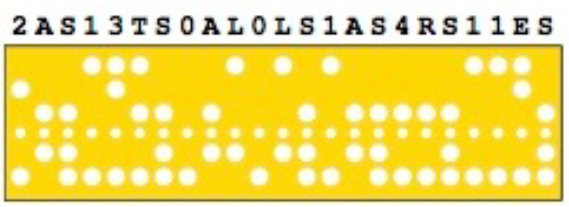
\includegraphics[scale = 0.3]{images/storia ling/Initial order.png}
    \caption{Initial order}
    \label{fig:Initial order}
\end{figure}

\paragraph{In sostanza:}

\begin{itemize}
    \item Alla fine degli anni '40 c'erano poche decine di programmatori e meno di 20 computers;
    \item Non esistevano corsi/tutorial di programmazione;
    \item Erano stati scritti pochi programmi.
\end{itemize}

\dfn{Short code}{Lo short code viene implementato nel '49 da Maurice Wilkes. Si tratta di un linguaggio
che permette di scrivere programmi in modo più semplice. Veniva assegnato uno specifico numero a 6 bit
per indicare variabili e simboli di un'equazione. Si scrisse anche un programma per il calcolo delle
equazioni da calcolare (una sorta di primitivo interprete).
}

Tra il 1948 e il 1950 Haskell Curry sviluppa la programmazione strutturata.
Tuttavia Curry non considerava la fase di analisi sintattica

\section{Gli anni '50}

\dfn{For}{Il costrutto for viene introdotto nel '51 da Rutishaur.
La sua idea permetteva di generare codice rilocabile.}

Nel 1950 l'italiano Corrado Böhm concepisce un linguaggio di alto livello e un metodo di traduzione in 
linguaggio macchina. Nel suo lavoro:

\begin{itemize}
    \item Vengono introdotti "if then else" e "goto";
    \item Gli statement di assegnamento;
    \item Le subroutine;
    \item Un compilatore scritto nello stesso linguaggio dei programmi che deve tradurre.
\end{itemize}

Il compilatore di Böhm genera codice proporzionalmente al numero di passi da eseguire. Inoltre il linguaggio
di Böhm è universale (tuttavia è solo su carta).

\subsection{AUTOCODE}

\dfn{AUTOCODE}{
Il primo compilatore degno di questo nome viene svippato nel 1953 da Alick Glennie che noto che si poteva
usare lo stesso computer per tradurre un programma e far girare il programma sullo stesso computer. AUTOCODE
era complicato e il suo compilatore era composto da 750 istruzioni.}

AUTOCODE:

\begin{itemize}
    \item Rendeva più veloce e semplice la programmazione;
    \item Costituiva una perdita di efficienza del 10\% rispetto al linguaggio macchina.
\end{itemize}

Ma il lavoro di Glennie non ebbe il successo sperato poichè in quegli anni il focus non era tanto sullo scrivere un programma
ma sul fatto che i calcolatori si rompessero continuamente.

Negli anni '50 si sviluppa l'idea di pseudo-codice e si parlava di automatic coding invece che di compilatori.

\subsection{Gli anni dal '54 al '56}

In queglu anni si stava tenendo il SIMATIC (Symposium on the Mechanization of Thought Processes) in cui si discuteva
delle proprie scoperte.

\begin{itemize}
    \item Nel 1954 si sviluppa il primo assembler moderno, il SOAP;
    \item Tra il 1954 e il 1956 alla Boeing Airplane Company di Seattle
    viene sviluppato il sistema BACAIC, in cui espressioni algebriche
    vengono tradotte in subroutine di linguaggio macchina;
    \item Enton
    Elsworth lavora ad un sistema per la traduzione di equazioni
    algebriche in linguaggio macchina (dell’IBM 701), e chiama il suo
    sistema Kompiler;
    \item Viene messo a punto ADES, il primo linguaggio di programmazione imperativo;
    \item Nel 1956 , per IBM 650, viene sviluppato il compilatore IT.
\end{itemize}

\dfn{IT}{IT funzionava in due fasi:
\begin{enumerate}
    \item Veniva generato codice assembler intermedio;
    \item Da quel codice veniva generato codice macchina
\end{enumerate}
IT permetteva di scrivere in un linguaggio semplice con un'implementazione efficiente.}

\subsection{Il FORTRAN}

\dfn{FORTRAN}{Nel 1957 il FORTRAN fa la sua comparsa. All'inizio del 1954 John Backus,
Harlan Herrick e Irving Ziller iniziano a lavorare su un linguaggio di programmazione. 
In quegli anni i programmi venivano scritti o in assembler o in linguaggio macchina, per
cui non si pensava che il FORTRAN potesse avere successo.}

\paragraph{Specifiche:}

\begin{itemize}
    \item Avrebbe dovuto essere facile scrivere programmi in FORTRAN e sarebbe dovuto essere
    efficiente;
    \item Avrebbe dovuto essere facile da imparare;
    \item Non doveva essere svincolato dall'hardware (in quanto linguaggio di IBM).
\end{itemize}

Il manuale del FORTRAN aveva una grafica professionale, ma era pieno di errori e incompleto.
Tuttavia il FORTRAN influenzo la maggior parte dei linguaggi successivi e fino agli anni '70
fu utilizzato come standard per applicazioni scientifiche.

\subsection{LISP}

\dfn{LISP}{Nel 1958 fa il suo debutto il LISP. Fu il primo dei linguaggi funzionali. Nasce per la manipolazione
di espessioni simboliche con l'uso del concetto di "ricorsione". Inoltre il LISP usava sia liste che alberi.
Offriva un garbage collector e un sistema di tipi dinamico. Permetteva la meta-programmazione.}

\begin{itemize}
    \item Viene usata una notazione polacca (prefissa);
    \item Alcuni operatori potevano venire implementati direttamente in linguaggio macchina.
\end{itemize}

\nt{Alcune parti di LISP erano codificate in FORTRAN}

In LISP tutto veniva rappresentato da liste concatenate. La lista concatenata a destra è la rappresentazione interna
dei dati.

\subsection{COBOL}

\dfn{COBOL}{
    Il COBOL (COmmon Business Oriented Language) fu concepito per applicazioni di tipo
    amministrativo e commerciale. Il COBOL aveva una sintassi "english-like", ciò lo rendeva
    facilmente comprensibile. Esempio:
    \begin{center}
        ADD A TO B GIVING C
    \end{center}
    Il COBOL venne sviluppato dal CODASYL (Conference on Data Systems Languages) e il DoD (Department of Defense)
    USA obbligo le compagnie produttrici di computer a fornire il COBOL nelle loro installazioni.
}

\cor{La sintassi del COBOL}{
    La sintassi del COBOL fu il risultato di un processo decisionale influenzato da 
    FLOW-MATIC (di Grace Hopper) e dall'IBM COMTRAN (di Bob Bemer)\footnote{Molto marginalmente.}.
}

\paragraph{Gli obiettivi:}

\begin{itemize}
    \item doveva essere portatile;
    \item doveva essere efficiente;
    \item doveva essere facilmente comprensibile e utilizzabile.
\end{itemize}

Ma il COBOL non fu recepito bene dalla comunità informatica: non si consideravano i programmatori
COBOL dei veri programmatori. Inoltre il COBOL non era adatto per applicazioni scientifiche.
Ai giorni nostri il COBOL è quasi del tutto scomparso.

\section{Gli anni '60}

\subsection{ALGOL 60}

\dfn{L'ALGOL 60}{
    L'ALGOL 60 (ALGOrithmic Language 1960) fu frutto di una collaborazione tra l'ACM (Association for Computing Machinery)
    e l'IFIP (International Federation for Information Processing). L'ALGOL 60 era molto legato
    all'hardware sottostante.
}

\nt{Tony Hoare\footnote{Inventore del Quicksort e del puntatore NULL} noto che l'ALGOL 60
era molto più avanti rispetto ai linguaggi dell'epoca.}

\paragraph{ALGOL 60 introduce:}

\begin{itemize}
    \item \textbf{call by value} (per i parametri);
    \item \textbf{call by name} (per le variabili);
    \item \textbf{call by reference} (per i parametri, passaggio di un puntatore);
\end{itemize}

L'ALGOL è il primo linguaggio a richiedere esplicitamente il tipo delle variabili, Inoltre
viene introdotta la distinzione tra assegnamento e uguaglianza. Oltre a qeusto si introducono
le prime primitive di controllo strutturate: if then else, while loop e for. Si introducono anche i blocchi di istruzioni:
\begin{center}
    BEGIN ... END
\end{center}

L'ALGOL per via del pesante utilizzo di GOTO consentiva programmazione non strutturata. Ciò
rende il codice meno leggibile.

\dfn{Spaghetti code}{
    Spaghetti code indica codice non strutturato e "ingarbugliato", difficilmente leggibile.   
}

\subsection{La Backus-Naur Form (BNF)}

\dfn{Backus-Naur Form (BNF)}{
    La BNF è una notazione per grammatiche context free. Viene usata per descrivere la
    sintassi dei linguaggi di programmazione e, essendo un metà linguaggio, può essere
    usata per descrivere se stessa.
}

\nt{Tutto ciò viene spiegato nel corso "Linguaggi formali e traduttori"}

\dfn{Panini Backus Form}{
    La Panini Backus Form è una versione ridotta della BNF. 
}

\cor{I parsificatori}{
    I parsificatori sono programmi che leggono un testo e lo analizzano per determinare
    la sua struttura grammaticale. ALGOL porto alla creazione di un parsificatore (LL). 
    Nel 1965, Donald Knuth sviluppa un altro parsificatore (LR), ma solo alla fine degli anni '60
    verranno messi a punto dei parsificatori efficienti.
}

\subsection{BASIC}

\dfn{Basic (Beginner's All-purpose Symbolic Instruction Code)}{
    Il BASIC nasce nel 1964 da un progetto di John Kemeny e Thomas Kurtz. Il BASIC era
    un linguaggio di programmazione semplice e facile da imparare. Il suo obiettivo era
    quello di consentire a studenti, non di informatica, di scrivere programmi.
}

\nt{Il BASIC inizia a diffondersi negli anni '70 con la diffusione dei "micro-computers".
In alcuni casi il BASIC diventava l'ambiente di lavoro del PC (un po' come la shell).}

Il BASIC era sufficientemente ad alto livello da poter essere utilizzato da chiunque ed
ebbe diffusione come linguaggio didattico. Ma anche il BASIC fu guardato con sufficienza
da molti informatici: Dijstra sosteneva che fosse inutile insegnare a programmare a gente 
che era stata esposta al COBOL o al BASIC.

\dfn{Visual BASIC}{
    Il visual BASIC fu introdotto da Microsoft nel 1991 sebbene fu utilizzato molto poc
    a causa della diffusione di linguaggi più potenti.
}

Altre varianti furono:
\begin{itemize}
    \item Altair BASIC;
    \item Game BASIC (poi ridenominato Integer BASIC);
    \item Applesoft BASIC.
\end{itemize}

\subsection{La questione del GOTO}

\thm{Bohm-Jacopini}{
    Il teorema ha diverse formulazioni equivalenti, ma sostanzialmente
asserisce che qualsiasi funzione computabile può essere calcolata da
un programma costituito esclusivamente da una combinazione di:
\begin{itemize}
    \item Sequenze di istruzioni eseguite una dopo l’altra;
    \item Istruzioni di selezione (del tipo if then else);
    \item Istruzioni di iterazione (del tipo while do).
\end{itemize}

}

\nt{In sostanza il teorema dimostrava che il GOTO poteva essere messo da parte.}

Nel 1968, Dijstra critica l'uso del GOTO in una lettera alle Communication of the ACM. 
Successivamente, nel 1974, Knuth mostra che in alcuni casi il GOTO era la scelta migliore.
Ne manuale di Brian Kernigham e Dennis Ritchie osservano che il GOTO era necessario per 
gestire alcuni casi di errore.

\subsection{Il Simula}

\dfn{Simula I}{
    Il Simula I nasce nel 1966 da un progetto di Kristen Nygaard e Ole-Johan Dahl. Il Simula I
    è il primo linguaggio ad oggetti. Il suo scopo principale era quello di gestire simulazioni.
}

\nt{Dahl e Nygaard si ispirarono al concetto di record class introdotto da Hoare nell'ALGOL 60.}

\dfn{Simula 67}{
    Il Simula 67 è la seconda versione del Simula. Il Simula 67 è il primo linguaggio ad oggetti
    a essere usato in ambito commerciale. Il Simula 67 introduce il concetto di classe e di
    sottoclasse. Le istanzee di una classe sono dette oggetti e l'operazione new permette di
    creare un oggetto. In Simula 67 erano anche presenti i puntatori (chiamati ref) ai record di attivazione (oggetti).
}

\nt{Per questi motivi si introduce un meccanismo di garbage collection.}

Il Simula 67 introduce anche la data abstraction e l'ereditarietà. Uno degli utilizzi del simula
era la modellazione di sistemi concorrenti.

\section{Gli anni '70}

\subsection{Pascal}

\dfn{Pascal}{
    Il Pascal nasce nel 1970 da un progetto di Niklaus Wirth. Può essere considerato un successore
    dell'ALGOL. Vengono introdotti i puntatori e il tipo CHAR. Il Pascal incoraggia la costruzione
    di procedure chiare, usa strutture dati dinamiche, call by value e call b reference.
    Un'altra caratteristica era il suo sistema di tipi molto ricco, ma molto rigido\footnote{Con type
    checking in fase di compilazione}.
}

\paragraph{Obiettivi:}

\begin{itemize}
    \item Semplicità;
    \item Chiarezza;
    \item Efficienza;
    \item Scrittura di programmi complessi.
\end{itemize}

Il compilatore del Pascal non generava direttamente codice macchina, ma generava un codice intermedio:
il P-Code. Il P-Code era un linguaggio assembly portabile. Il P-Code veniva interpretato da una
macchina virtuale. Verso la fine degli anni '70 il Pascal era ormai in uso e insegnato nelle università.

L'Educational Testing Service (ETS), rese il Pascal il linguaggio standard per i test AP (Advanced Placement).
Nel 1983 Hejlsberf sviluppa il Turbo Pascal, un compilatore per PC. Il Turbo Pascal era un compilatore
molto efficiente e permetteva di scrivere programmi in Pascal in modo molto veloce (diventò lo standard dei PC).

Apple utilizzo il Pascal come linguaggio di riferimetno per il suo sistema operativo così come Microsoft.
Tuttavia il Pascal declino in favore di C e di UNIX.

\subsection{Il Prolog}

\dfn{Il Prolog}{
    Il Prolog (PROgrammation en LOGique) nasce nel 1972 da un progetto di Alain Colmerauer e Philippe Roussel. Il Prolog è un linguaggio
    dichiarativo basato sulla logica del primo ordine. Il Prolog è un dimostratore automatico di teoremi. 
}

\nt{I dimostratori automatici di teoremi sono utilizzati nel corso di "Metodi formali per l'informatica" e
nella parte da +3 CFU del corso di "Linguaggi e paradigmi".}

\dfn{The Fifth Generation Computer Systems (FGCS)}{
Nel 1981 il governp giapponese lancia il progetto FGCS. L'obiettivo 
era quello di sviluppare un computer sfruttando il parallelismo,
il linguaggio naturale e AI, per cui il Prolog era particolarmente adatto.
Questo progetto ebbe molta risonanza a livello mondiale e portò
i vari governi a investire in ricerca.
}

\nt{Nel 1982  Ehud Shapiro sviluppa il linguaggio Concurrent Prolog.}

Le macchine della quinta generazione dovevano eseguire operazioni logiche
che sarebbero state valutate in Logic Inferences Per Second (LIPS).

Dopo 10 anni di tentativi e investimenti il progetto FGCS fallisce:
\begin{itemize}
    \item I processori RISC erano più veloci delle macchine FGCS;
    \item Lo sfruttamento del parallelismo era più difficile del previsto;
    \item Il paradigma logico era difficile da usare.
\end{itemize}

\subsection{Lo Smalltalk}

\dfn{Smalltalk}{
    Lo Smalltalk nasce nel 1972 da un progetto di Alan Kay. 
    Diverse versioni furono sviluppate da Dan Ingalls e Adele Goldberg.
    Lo Smalltalk fornì il primo ambiente di programmazione
    dotato di interfaccia grafica (GUI), implementato sullo
    Xerox Alto. 

    Lo Smalltalk è un linguaggio orientato agli oggetti in cui esistono
    \textit{solo} oggetti. Gli oggetti hanno dati privati e comunicano
    mediante metodi. Si utilizzava un sistema di tipi dinamico. 
}

\nt{Alan Kay concepisce anche il Dynabook, un computer portatile.}

Kay divide i linguaggi in due categorie:

\begin{itemize}
    \item quelli prodotti da comitati;
    \item quelli prodotti da individui: questi sono i linguaggi più innovativi.
\end{itemize}

\subsection{ADA: il linguaggio definitivo}

\dfn{ADA}{
    Il progetto parte nel 1974 al Department of Defense (DoD) USA per
    standardizzare i linguaggi di programmazione. Dopo 3 anni venne
    scelto il progetto di Jean Ichbiah che, con i report di 15 nazioni,
    sviluppa il linguaggio ADA, in onore di Ada Lovelace. 
    Secondo Ichbiah sarebbero sopravvissuti solo 2 linguaggi: ADA e LISP.
    Ma i primi compilatori ADA erano lenti.

    L'ADA prendeva caratteristiche dall'ALGOL (strutture di controllo
    e sintassi), dal Pascal (Sistema di tipi) e dal SIMULA (gestione
    concorrenza e parallelismo).
}

\nt{Tuttavia non era orientato agli oggetti al lancio, ma solo dal 1995.}

\section{Il C}

Se si considera la diffusione il C è il linguaggio più importante della storia.
Il C era estremamente efficiente e portabile. 
\dfn{Il C}{
A metà degli anni '60 i laboratori Bell insieme al MIT e alla General Electric
iniziarono il progetto di un nuovo sistema operativo (MULTICS). 
Dennis Ritchie, Ken Thompson e Brian Kernigham erano tra gli
sviluppatori del MULTICS, ma nel 1969 il progetto venne abbandonato.
Così Thompson e Ritchie svilupparono il sistema operativo UNIX (come scherzo
nei confronti di MULTICS). Inizialmente era scritto in assembler, poi in B, 
predecessore del C. 

Tra il 1971 e il 1972 Ritchie modifica il B e nasce il C (inizialmente NB o New B).

}

\paragraph{Il C era dotato di:}

\begin{itemize}
    \item Portabilità;
    \item Efficienza;
    \item Modularità;
    \item Compattezza;
    \item Tipi flessibili;
    \item Gestione efficiente della memoria;
    \item Bitwise programming.
\end{itemize}

\nt{Si deve a Kernigham il concetto di "Hello World".}

\dfn{The obfuscated C code}{
    L'international obfuscated C code contest è un concorso di programmazione
    che consiste nel scrivere il programma più incomprensibile in C che funziona.
}


\subsection{La nascita del C++}

\dfn{Il C++}{
    Il C++ nasce nel 1979 da un progetto di Bjarne Stroustrup. Si
    tratta di un'evoluzione del C orientata all'object-oriented.
}

\nt{Nel 2001 viene rilasciato il D, un'evoluzione del C++ influenzata
da Java, Ruby e Python.}

\subsection{Objective-C e C-Sharp}

\dfn{Objective-C}{
    L'Objective-C nasce nel 1983 da un progetto di Brad Cox e Tom Love. 
    Si tratta di un'evoluzione del C orientata all'object-oriented.
}

\dfn{C-Sharp}{
    Il C-Sharp nasce nel 2000 da un progetto di Microsoft. 
    Si tratta di un'evoluzione del C orientata all'object-oriented.
    È stato sviluppato per la piattaforma .NET.
}

\section{Gli anni '90: il Web e Java}

Nel 1993 avvenne un evento che cambiò il mondo dell'informatica: il World Wide Web. 
Al NCSA (National Center for Supercomputing Applications) viene sviluppato il Mosaic,
il primo browser grafico. Il Mosaic rendeva le pagine web più accessibili e più facili
da creare. Questo browser metteva a disposizione degli utenti una enorme quantità di
informazioni.Negli anni '90 nascono anche le applet: piccoli programmi che venivano
eseguiti all'interno del browser il cui linguaggio era WORA (Write Once Run Anywhere).
Questo linguaggio diventerà poi il Java.

\dfn{Java}{
    Il Java nasce a partire dal 1990 da un progetto di Sun Microsystems\footnote{
        Azienda che sviluppò Solaris e NFS.
    }. Fu rilasciato nel 1995 insieme al browser HotJava (per eseguire le applet).
    Successivamente tutti gli altri browser implementarono una Java Virtual Machine.
}

\section{Verso il 21esimo secolo : i linguaggi di scripting}

\dfn{Linguaggio di scripting}{
    Un linguaggio di scripting è un linguaggio di programmazione interpretato
    che viene utilizzato per scrivere script. Gli script sono programmi che
    vengono eseguiti da un interprete. Per esempio il linguaggio bash è un
    linguaggio di scripting.
}

\nt{In linea di principio qualsiasi linguaggio può essere usato come linguaggio
di scripting, ma in pratica richiederebbero un interprete.}

\paragraph{Linguaggi di scripting general purpose:}

\begin{itemize}
    \item coniugano le caratteristiche dei classici linguaggo di programmazione;
    \item prototipazione veloce.
\end{itemize}

\dfn{Perl}{
    Il Perl nasce nel 1987 da un progetto di Larry Wall come linguaggio
    di scripting per l'elaborazione di testi e file. È usato per scrivere
    script per il web, per l'amministrazione di sistemi e per l'elaborazione
    di testi. 
}

\nt{Di recente, il Perl, viene insegnato nel corso di "Bioinformatica" alla magistrale.}

\section{Digressione: altri linguaggi}


\dfn{Python}{
    Il Python nasce nel 1991 da un progetto di Guido van Rossum. Possiede caratteristiche
    object-oriented e funzionali e ha una sintassi semplice e chiara.
}

\dfn{PHP}{
    Il PHP (PHP: Hypertext Preprocessor) nasce nel 1994 da un programma di Rasmus Lerdorf.
    È un linguaggio di scripting per la programmazione web. 
}

\dfn{JavaScript}{
    Il JavaScript nasce nel 1995 (sviluppato in 10 giorni) da un progetto di Brendan Eich. È un linguaggio di scripting
    per la programmazione web. Con JavaScript nasce una guerra tra Netscape e 
    Internet Explorer. 
}

\dfn{Ruby}{
    Il Ruby nasce nel 1995 da un progetto di Yukihiro Matsumoto. È un linguaggio di scripting
    orientato agli oggetti che doveva inglobare le caratteristiche migliori:
    \begin{itemize}
        \item la praticità del Perl;
        \item orientato agli oggetti cone lo Smalltalk;
        \item la semplicità del Lisp.
    \end{itemize}
}